\subsubsection*{Sparse-Grids and Uncertainty Quantification}

The mathematical component of this project will be based on new
developments combining sparse
grids~\parencite{BungartzGriebel2004}, reduced basis
methods~\parencite{LiebermanEtal2010,Peherstorfer2013,ChenSchwab2015,PeherstorferWillcox2015}
and uncertainty quantification. One of the main difficulties in the
study of current scientific models is the high dimensional spaces
involved, often both in the parameter and domain spaces, $\mathcal{P}$
and $\mathcal{D}$ respectively. This is a significant barrier for the
timely evaluation of models due to the `curse of dimensionality' in
which the cost scales exponentially with dimension. By using sparse
grids and reduced basis models we will be able to compute
\emph{surrogates of the full problem} which have significantly fewer
unknowns and are thus cheaper to compute whilst maintaining a high
order of accuracy. For example, a general approach would be to find a
lower dimensional manifold of the parameter space
$\mathcal{Q}\subset\mathcal{P}$ over which the model is most sensitive
using a proper orthogonal decomposition. A sparse grid surrogate of
the model over $\mathcal{Q}$ can also be computed in an offline phase,
so that in an online phase model solutions can be efficiently
estimated using the surrogate model. For many problems sparse grids
can also be used over $\mathcal{D}$ when computing solutions to the full
model to speed up the construction of a reduced basis. We will compute
sparse grid solutions via the `combination
technique'~\parencite{Griebel1990}. Figure~\ref{fig:sparse_grids}
depicts the combination technique, the equivalent sparse grid and the
corresponding full grid.

\begin{figure}
  \centering
  % Brendan: combination grid, sparse grid, fullgrid figure

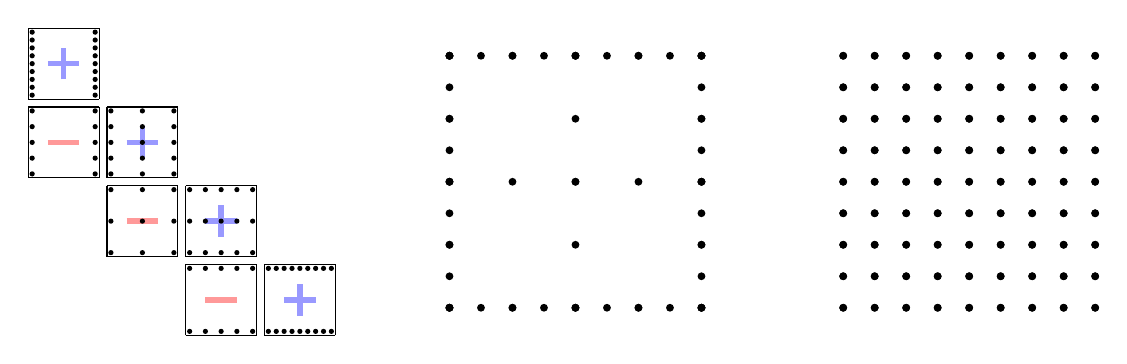
\begin{tikzpicture}%[scale=0.8]
%\scriptsize
%%% Draw squares around component grids
\foreach \i in {1,...,4}
{
	\pgfmathtruncatemacro{\x}{(\i - 1)};
	\draw[] (0.05+1.0*\x, 3.05-1.0*\x) -- (0.05+1.0*\x+0.9, 3.05-1.0*\x) {};
	\draw[] (0.05+1.0*\x, 3.05-1.0*\x) -- (0.05+1.0*\x, 3.05-1.0*\x+0.9) {};
	\draw[] (0.05+1.0*\x+0.9, 3.05-1.0*\x) -- (0.05+1.0*\x+0.9, 3.05-1.0*\x+0.9) {};
	\draw[] (0.05+1.0*\x, 3.05-1.0*\x+0.9) -- (0.05+1.0*\x+0.9, 3.05-1.0*\x+0.9) {};
	%%% optional plotting of coefficients
	\draw[blue!40,line width=0.7mm] (0.5+1.0*\x-0.2, 3.0+0.5-1.0*\x) -- (0.5+1.0*\x+0.2, 3.0+0.5-1.0*\x);
	\draw[blue!40,line width=0.7mm] (0.5+1.0*\x, 3.0+0.5-1.0*\x-0.2) -- (0.5+1.0*\x, 3.0+0.5-1.0*\x+0.2);
}
\foreach \i in {1,...,3}
{
	\pgfmathtruncatemacro{\x}{(\i - 1)};
	\draw[] (0.05+1.0*\x, 2.05-1.0*\x) -- (0.05+1.0*\x+0.9, 2.05-1.0*\x) {};
	\draw[] (0.05+1.0*\x, 2.05-1.0*\x) -- (0.05+1.0*\x, 2.05-1.0*\x+0.9) {};
	\draw[] (0.05+1.0*\x+0.9, 2.05-1.0*\x) -- (0.05+1.0*\x+0.9, 2.05-1.0*\x+0.9) {};
	\draw[] (0.05+1.0*\x, 2.05-1.0*\x+0.9) -- (0.05+1.0*\x+0.9, 2.05-1.0*\x+0.9) {};
	%%% optional plotting of coefficients
	\draw[red!40,line width=0.7mm] (0.5+1.0*\x-0.2, 2.0+0.5-1.0*\x) -- (0.5+1.0*\x+0.2, 2.0+0.5-1.0*\x);
}
%%% Combination grids
\foreach \i in {1,...,18} %2*9
{
	\pgfmathtruncatemacro{\y}{(\i - 1) / 2};
	\pgfmathtruncatemacro{\x}{\i - 1 - 2 * \y};
	\node[fill,circle,scale=0.2] at (0.1+0.8*\x,3.1+0.1*\y) {};
	\node[fill,circle,scale=0.2] at (3.1+0.1*\y,0.1+0.8*\x) {};
}
\foreach \i in {1,...,15} %3*5
{
	\pgfmathtruncatemacro{\y}{(\i-1)/3};
	\pgfmathtruncatemacro{\x}{\i-1-3*\y};
	\node[fill,circle,scale=0.2] at (1.1+0.4*\x,2.1+0.2*\y) {};
	\node[fill,circle,scale=0.2] at (2.1+0.2*\y,1.1+0.4*\x) {};
}
\foreach \i in {1,...,10} %2*5
{
	\pgfmathtruncatemacro{\y}{(\i-1)/2};
	\pgfmathtruncatemacro{\x}{\i-1-2*\y};
	\node[fill,circle,scale=0.2] at (0.1+0.8*\x,2.1+0.2*\y) {};
	\node[fill,circle,scale=0.2] at (2.1+0.2*\y,0.1+0.8*\x) {};
}
\foreach \i in {1,...,9} %3*3
{
	\pgfmathtruncatemacro{\y}{(\i - 1) / 3};
	\pgfmathtruncatemacro{\x}{\i - 1 - 3 * \y};
	\node[fill,circle,scale=0.2] at (1.1+0.4*\x,1.1+0.4*\y) {};
}
%%% Sparse grid
\foreach \i in {1,...,18} %2*9
{
	\pgfmathtruncatemacro{\y}{(\i - 1) / 2};
	\pgfmathtruncatemacro{\x}{\i - 1 - 2 * \y};
	\node[fill,circle,scale=0.3] at (5.4+3.2*\x,0.4+0.4*\y) {};
	\node[fill,circle,scale=0.3] at (5.4+0.4*\y,0.4+3.2*\x) {};
}
\foreach \i in {1,...,15} %3*5
{
	\pgfmathtruncatemacro{\y}{(\i-1)/3};
	\pgfmathtruncatemacro{\x}{\i-1-3*\y};
	\node[fill,circle,scale=0.3] at (5.4+1.6*\x,0.4+0.8*\y) {};
	\node[fill,circle,scale=0.3] at (5.4+0.8*\y,0.4+1.6*\x) {};
}
%%% Full grid
\foreach \i in {1,...,81} %9*9
{
	\pgfmathtruncatemacro{\y}{(\i - 1) / 9};
	\pgfmathtruncatemacro{\x}{\i - 1 - 9 * \y};
	\node[fill,circle,scale=0.3] at (10.4+0.4*\x,0.4+0.4*\y) {};
	\node[fill,circle,scale=0.3] at (10.4+0.4*\y,0.4+0.4*\x) {};
}
\end{tikzpicture}  
  \caption{Combination grids on the left (with coefficients, marked with
    a blue plus for $+1$ and red minus for $-1$), sparse grid in the
    middle, full grid on the right. Note the marked reduction in the number of 
    grid points for the sparse grid relative to the full grid. 
   This is even more pronounced in higher dimensions.}
  \label{fig:sparse_grids}
\end{figure}

Propagating uncertainty in scientific models which are high
dimensional and/or expensive to compute is a significant challenge.
For models which are not stochastic in nature, and thus have no means
of directly quantifying uncertainty, one must typically estimate
statistical moments via Monte Carlo methods or quadrature rules. For
high dimensional problems it has been shown that sparse grids can
estimate these moments faster and more accurately than traditional
Monte Carlo methods when the probability density functions are
sufficiently
smooth~\parencite{JakemanRoberts2013,FranzelinDiehlPfluger2014}.
Despite the advantages of reduced basis methods, the manifold
$\mathcal{Q}$ is still sufficiently high dimensional that the
quantification of uncertainty remains a challenge due to the sheer
number of function evaluations required. This is particularly true
when the quantification of uncertainty in a model is a component of an
optimisation algorithm. As such it is important to continue to
develop efficient numerical methods for uncertainty quantification
for high dimensional problems. Replacing the full model with a reduced
basis model also adds additional error and uncertainties. One needs to
have some idea what the model outcomes may be for parameters not lying
on the lower dimensional manifold $\mathcal{Q}$. An important part of
developing reduced models is `verifying' the model, by bounding the
error of the surrogate for example. By using ensemble methods,
multifidelity models~\parencite{NgWillcox2014} and gradient enhanced
approximation~\parencite{deBaarHarding2015,Jakeman2015} we hope to
improve the verification and propagation of uncertainties in models.
Incorporating ideas from `Kriging' (Gaussian process regression), a
feature of which is having confidence intervals over an interpolant,
together with sparse-grid interpolation, we will be able to express
uncertainties explicitly in the surrogate model.

